\documentclass[12pt,a4paper]{report}
\usepackage[utf8]{inputenc}
\usepackage[T1]{fontenc}
\usepackage{geometry}
\usepackage{graphicx}
\usepackage{hyperref}
\usepackage{listings}
\usepackage{xcolor}
\usepackage{tikz}
\usepackage{booktabs}
\usepackage{longtable}
\usepackage{fancyhdr}
\usepackage{tocloft}
\usepackage{enumitem}
\usepackage{amsmath}
\usepackage{float}
\usetikzlibrary{shapes.geometric, arrows, positioning, fit}

\geometry{margin=1in}

% Define colors
\definecolor{codegreen}{rgb}{0,0.6,0}
\definecolor{codegray}{rgb}{0.5,0.5,0.5}
\definecolor{codepurple}{rgb}{0.58,0,0.82}
\definecolor{backcolour}{rgb}{0.95,0.95,0.92}
\definecolor{djangogreen}{RGB}{12,75,51}

% Code listing style
\lstdefinestyle{mystyle}{
    backgroundcolor=\color{backcolour},   
    commentstyle=\color{codegreen},
    keywordstyle=\color{magenta},
    numberstyle=\tiny\color{codegray},
    stringstyle=\color{codepurple},
    basicstyle=\ttfamily\footnotesize,
    breakatwhitespace=false,         
    breaklines=true,                 
    captionpos=b,                    
    keepspaces=true,                 
    numbers=left,                    
    numbersep=5pt,                  
    showspaces=false,                
    showstringspaces=false,
    showtabs=false,                  
    tabsize=2,
    frame=single
}
\lstset{style=mystyle}

% Header and Footer
\pagestyle{fancy}
\fancyhf{}
\fancyhead[L]{\leftmark}
\fancyhead[R]{Student Tour Management System}
\fancyfoot[C]{\thepage}

% Hyperlink setup
\hypersetup{
    colorlinks=true,
    linkcolor=blue,
    filecolor=magenta,      
    urlcolor=cyan,
    pdftitle={Student Tour Management System Documentation},
    pdfauthor={Project Team},
}

% Title Page Information
\title{
    \vspace{2cm}
    \includegraphics[width=0.3\textwidth]{example-image}\\ % Replace with your logo
    \vspace{1cm}
    \textbf{\Huge Student Tour Management System}\\
    \vspace{0.5cm}
    \Large Technical Documentation \& User Guide\\
    \vspace{1cm}
    \large Django Web Application
}
\author{
    \textbf{Development Team}\\
    \vspace{0.3cm}
    University Name
}
\date{\today}

\begin{document}

% Title Page
\maketitle
\thispagestyle{empty}
\newpage

% Table of Contents
\tableofcontents
\newpage

% List of Figures
\listoffigures
\newpage

% List of Tables
\listoftables
\newpage

%============================================
% CHAPTER 1: PROJECT OVERVIEW
%============================================
\chapter{Project Overview}

\section{Introduction}
The \textbf{Student Tour Management System} is a comprehensive web application developed using the Django framework. This system is designed to facilitate the management of student tours, travel packages, and bookings for educational institutions.

\subsection{Purpose}
The primary objectives of this system are:
\begin{itemize}[noitemsep]
    \item Provide students with an easy-to-use platform to browse and book tour packages
    \item Enable administrators to manage tour packages, bookings, and student requests
    \item Streamline the payment verification process
    \item Maintain a centralized database for all travel-related activities
    \item Provide communication channels between students and administrators
\end{itemize}

\subsection{Scope}
This system encompasses:
\begin{itemize}[noitemsep]
    \item User authentication and role-based access control
    \item Tour package management (Study Tours, Cycling, University Programs)
    \item Tourist spot information management
    \item Booking and payment processing
    \item Travel request submission and approval workflow
    \item Contact message management
\end{itemize}

\section{Technology Stack}
\begin{table}[H]
\centering
\caption{Technology Stack}
\label{tab:tech-stack}
\begin{tabular}{|l|l|p{7cm}|}
\hline
\textbf{Component} & \textbf{Technology} & \textbf{Description} \\
\hline
Backend Framework & Django 5.2.9 & Python web framework for rapid development \\
\hline
Database & SQLite3 & Lightweight relational database \\
\hline
Frontend & HTML5, CSS3, Bootstrap & Responsive user interface \\
\hline
Image Processing & Pillow 12.0.0 & Python imaging library \\
\hline
Web Server & Gunicorn 23.0.0 & Python WSGI HTTP Server \\
\hline
Static Files & WhiteNoise 6.11.0 & Static file serving for production \\
\hline
\end{tabular}
\end{table}

\section{System Requirements}
\subsection{Software Requirements}
\begin{itemize}[noitemsep]
    \item Python 3.10 or higher
    \item pip (Python package manager)
    \item Git (for version control)
    \item Virtual environment support
\end{itemize}

\subsection{Hardware Requirements}
\begin{itemize}[noitemsep]
    \item Minimum 2GB RAM
    \item 500MB free disk space
    \item Internet connection for deployment
\end{itemize}

%============================================
% CHAPTER 2: SYSTEM ARCHITECTURE
%============================================
\chapter{System Architecture}

\section{Django MVT Architecture}
Django follows the \textbf{Model-View-Template (MVT)} architectural pattern, which is a variation of the traditional MVC pattern.

\begin{figure}[H]
\centering
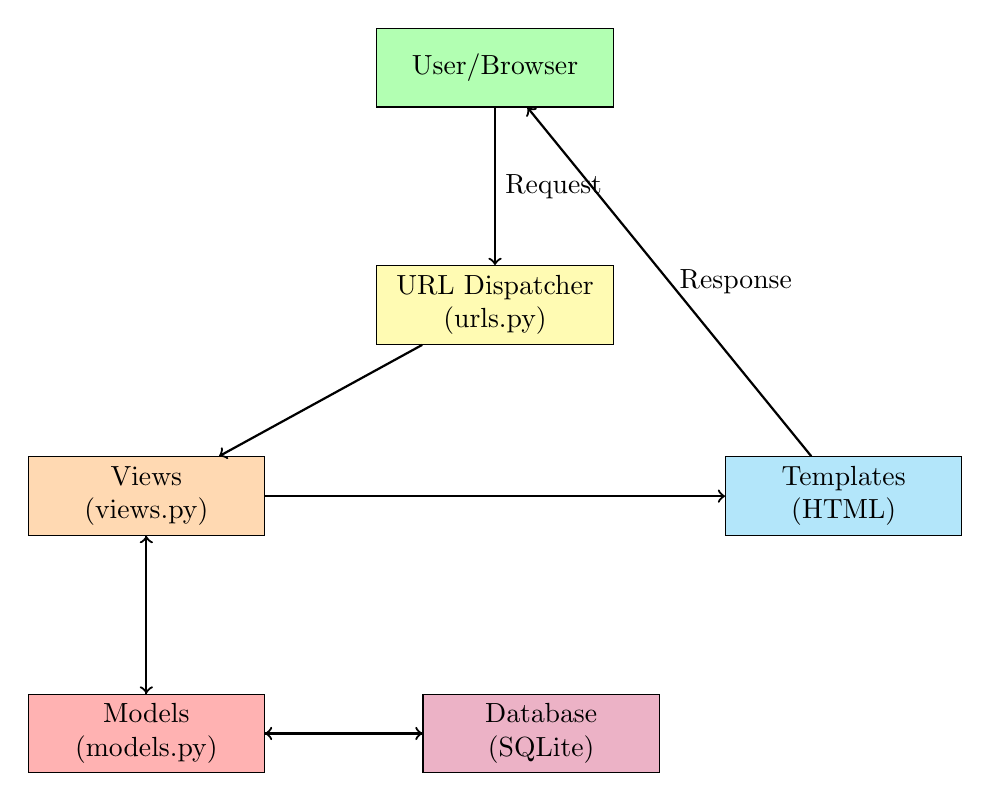
\begin{tikzpicture}[
    node distance=2cm,
    box/.style={rectangle, draw, minimum width=3cm, minimum height=1cm, align=center, fill=blue!20},
    arrow/.style={->, thick}
]
    % Nodes
    \node[box, fill=green!30] (user) {User/Browser};
    \node[box, fill=yellow!30, below=of user] (urls) {URL Dispatcher\\(urls.py)};
    \node[box, fill=orange!30, below left=of urls] (views) {Views\\(views.py)};
    \node[box, fill=red!30, below=of views] (models) {Models\\(models.py)};
    \node[box, fill=purple!30, right=of models] (db) {Database\\(SQLite)};
    \node[box, fill=cyan!30, below right=of urls] (templates) {Templates\\(HTML)};
    
    % Arrows
    \draw[arrow] (user) -- (urls) node[midway, right] {Request};
    \draw[arrow] (urls) -- (views);
    \draw[arrow] (views) -- (models);
    \draw[arrow] (models) -- (db);
    \draw[arrow] (db) -- (models);
    \draw[arrow] (models) -- (views);
    \draw[arrow] (views) -- (templates);
    \draw[arrow] (templates) -- (user) node[midway, right] {Response};
\end{tikzpicture}
\caption{Django MVT Architecture Flow}
\label{fig:mvt-arch}
\end{figure}

\subsection{Component Description}
\begin{description}
    \item[Model:] Defines the data structure and handles database operations. Located in \texttt{models.py} files.
    \item[View:] Contains the business logic and handles user requests. Located in \texttt{views.py} files.
    \item[Template:] Renders the HTML response to the user. Located in the \texttt{templates/} directory.
    \item[URL Dispatcher:] Routes incoming requests to appropriate views. Located in \texttt{urls.py} files.
\end{description}

\section{Project Structure}
\begin{lstlisting}[language=bash, caption=Project Directory Structure]
os_djangopro/
|-- manage.py                    # Django management script
|-- db.sqlite3                   # SQLite database file
|-- requirements.txt             # Python dependencies
|-- Procfile                     # Deployment configuration
|-- runtime.txt                  # Python version for hosting
|
|-- os_djangopro/               # Main project configuration
|   |-- __init__.py
|   |-- settings.py             # Project settings
|   |-- urls.py                 # Main URL configuration
|   |-- wsgi.py                 # WSGI application
|   |-- asgi.py                 # ASGI application
|
|-- accounts/                   # User authentication app
|   |-- models.py               # User-related models
|   |-- views.py                # Authentication views
|   |-- forms.py                # User forms
|   |-- urls.py                 # URL routes
|
|-- tourist_spots/              # Tour management app
|   |-- models.py               # Tour package models
|   |-- views.py                # Tour management views
|   |-- forms.py                # Tour forms
|   |-- urls.py                 # URL routes
|
|-- templates/                  # HTML templates
|-- static/                     # Static files (CSS, JS, images)
|-- media/                      # User-uploaded files
\end{lstlisting}

\section{Application Modules}
The system consists of two main Django applications:

\subsection{Accounts App}
Responsible for:
\begin{itemize}[noitemsep]
    \item User registration and authentication
    \item Role-based access (Student/Admin)
    \item Study tour management
    \item Booking management for study tours
    \item Contact message handling
\end{itemize}

\subsection{Tourist Spots App}
Responsible for:
\begin{itemize}[noitemsep]
    \item Tourist spot information management
    \item Tour package management (Study Tour, Cycling, University Programs)
    \item Package booking system
    \item Payment processing
    \item Travel request management
\end{itemize}

%============================================
% CHAPTER 3: DATABASE DESIGN
%============================================
\chapter{Database Design}

\section{Database Overview}
The system uses SQLite3 as the database backend. SQLite is a lightweight, file-based database that is perfect for development and small to medium-scale deployments.

\section{Entity Relationship Diagram (ERD)}
The ERD shows the relationships between different entities in the system.

\begin{figure}[H]
\centering
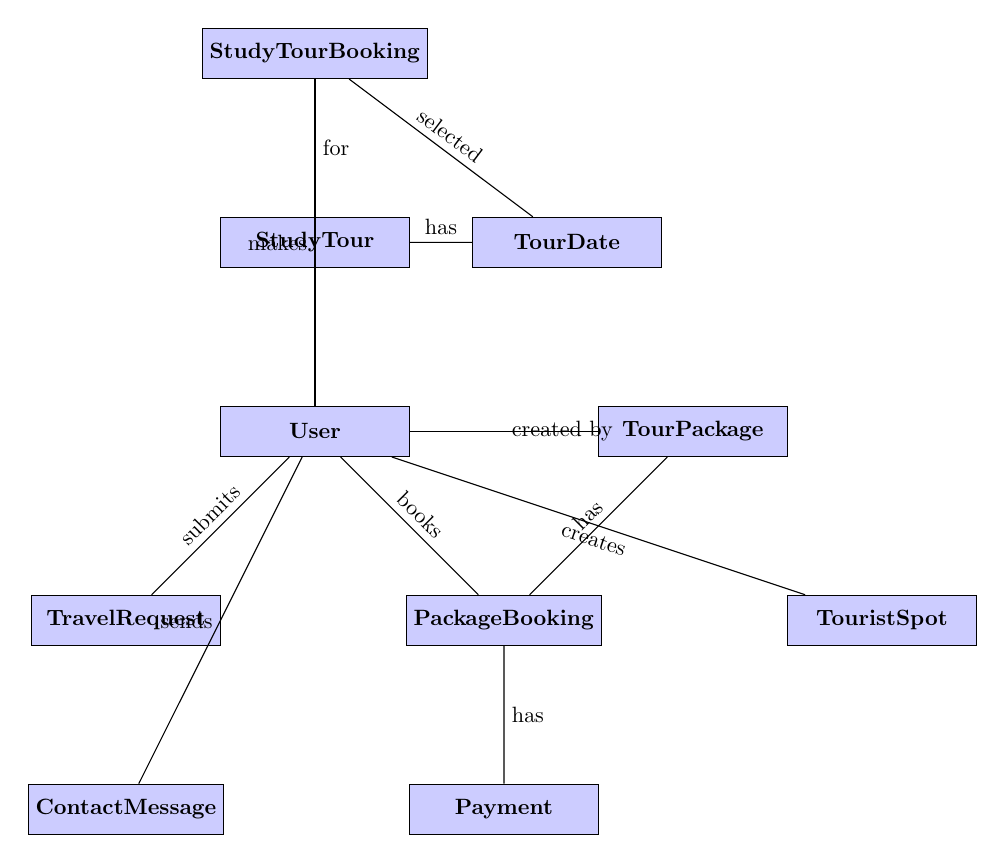
\begin{tikzpicture}[
    entity/.style={rectangle, draw, fill=blue!20, minimum width=3cm, minimum height=0.8cm},
    relationship/.style={diamond, draw, fill=yellow!30, aspect=2},
    attribute/.style={ellipse, draw, fill=green!10, minimum width=1.5cm, font=\small},
    scale=0.8, transform shape
]
    % User Entity
    \node[entity] (user) at (0,0) {\textbf{User}};
    
    % TourPackage Entity
    \node[entity] (package) at (6,0) {\textbf{TourPackage}};
    
    % PackageBooking Entity
    \node[entity] (booking) at (3,-3) {\textbf{PackageBooking}};
    
    % Payment Entity
    \node[entity] (payment) at (3,-6) {\textbf{Payment}};
    
    % TravelRequest Entity
    \node[entity] (request) at (-3,-3) {\textbf{TravelRequest}};
    
    % TouristSpot Entity
    \node[entity] (spot) at (9,-3) {\textbf{TouristSpot}};
    
    % ContactMessage Entity
    \node[entity] (contact) at (-3,-6) {\textbf{ContactMessage}};
    
    % StudyTour Entity
    \node[entity] (studytour) at (0,3) {\textbf{StudyTour}};
    
    % TourDate Entity
    \node[entity] (tourdate) at (4,3) {\textbf{TourDate}};
    
    % StudyTourBooking Entity
    \node[entity] (stbooking) at (0,6) {\textbf{StudyTourBooking}};
    
    % Relationships
    \draw[-] (user) -- node[above, sloped] {books} (booking);
    \draw[-] (package) -- node[above, sloped] {has} (booking);
    \draw[-] (booking) -- node[right] {has} (payment);
    \draw[-] (user) -- node[above, sloped] {submits} (request);
    \draw[-] (user) -- node[below, sloped] {creates} (spot);
    \draw[-] (user) -- node[left] {sends} (contact);
    \draw[-] (user) -- node[left] {makes} (stbooking);
    \draw[-] (studytour) -- node[above] {has} (tourdate);
    \draw[-] (studytour) -- node[right] {for} (stbooking);
    \draw[-] (tourdate) -- node[above, sloped] {selected} (stbooking);
    \draw[-] (package) -- node[right] {created by} (user);
\end{tikzpicture}
\caption{Entity Relationship Diagram}
\label{fig:erd}
\end{figure}

\section{Enhanced Entity Relationship Diagram (EER)}
The EER diagram extends the basic ERD by showing inheritance, specialization, and additional constraints.

\begin{figure}[H]
\centering
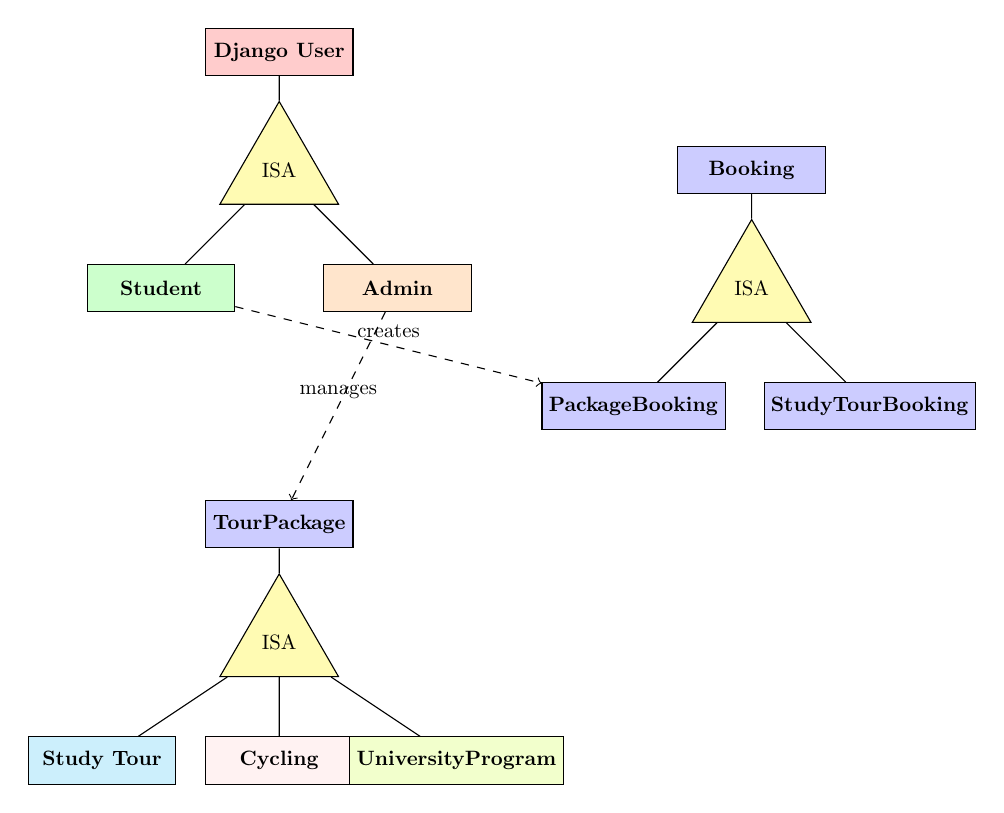
\begin{tikzpicture}[
    entity/.style={rectangle, draw, fill=blue!20, minimum width=2.5cm, minimum height=0.8cm},
    weak/.style={rectangle, draw, double, fill=blue!10, minimum width=2.5cm, minimum height=0.8cm},
    isa/.style={regular polygon, regular polygon sides=3, draw, fill=yellow!30, minimum size=1cm},
    scale=0.75, transform shape
]
    % Django User (Base)
    \node[entity, fill=red!20] (djangouser) at (0,8) {\textbf{Django User}};
    
    % ISA Triangle
    \node[isa] (isa1) at (0,6) {ISA};
    
    % Specialization
    \node[entity, fill=green!20] (student) at (-2,4) {\textbf{Student}};
    \node[entity, fill=orange!20] (admin) at (2,4) {\textbf{Admin}};
    
    % Lines
    \draw[-] (djangouser) -- (isa1);
    \draw[-] (isa1) -- (student);
    \draw[-] (isa1) -- (admin);
    
    % Booking Generalization
    \node[entity] (genbooking) at (8,6) {\textbf{Booking}};
    \node[isa] (isa2) at (8,4) {ISA};
    \node[entity] (pkgbooking) at (6,2) {\textbf{PackageBooking}};
    \node[entity] (stbooking) at (10,2) {\textbf{StudyTourBooking}};
    
    \draw[-] (genbooking) -- (isa2);
    \draw[-] (isa2) -- (pkgbooking);
    \draw[-] (isa2) -- (stbooking);
    
    % Tour Package Categories
    \node[entity] (tourpkg) at (0,0) {\textbf{TourPackage}};
    \node[isa] (isa3) at (0,-2) {ISA};
    \node[entity, fill=cyan!20] (studytour) at (-3,-4) {\textbf{Study Tour}};
    \node[entity, fill=pink!20] (cycling) at (0,-4) {\textbf{Cycling}};
    \node[entity, fill=lime!20] (uniprog) at (3,-4) {\textbf{University\\Program}};
    
    \draw[-] (tourpkg) -- (isa3);
    \draw[-] (isa3) -- (studytour);
    \draw[-] (isa3) -- (cycling);
    \draw[-] (isa3) -- (uniprog);
    
    % Relationships
    \draw[->, dashed] (student) -- node[above] {creates} (pkgbooking);
    \draw[->, dashed] (admin) -- node[above] {manages} (tourpkg);
\end{tikzpicture}
\caption{Enhanced Entity Relationship Diagram (EER)}
\label{fig:eer}
\end{figure}

\section{Database Tables}

\subsection{Accounts App Tables}

\begin{table}[H]
\centering
\caption{StudyTour Table}
\label{tab:studytour}
\begin{tabular}{|l|l|l|p{5cm}|}
\hline
\textbf{Field} & \textbf{Type} & \textbf{Constraints} & \textbf{Description} \\
\hline
id & BigAutoField & PK, Auto & Primary key \\
name & CharField(200) & NOT NULL & Tour name \\
description & TextField & NOT NULL & Detailed description \\
original\_price & Decimal(10,2) & NOT NULL & Original price \\
discounted\_price & Decimal(10,2) & NOT NULL & Discounted price \\
discount\_percentage & Integer & Default: 20 & Discount percentage \\
max\_students & Integer & Default: 25 & Maximum students allowed \\
is\_active & Boolean & Default: True & Active status \\
created\_at & DateTime & Auto & Creation timestamp \\
\hline
\end{tabular}
\end{table}

\begin{table}[H]
\centering
\caption{TourDate Table}
\label{tab:tourdate}
\begin{tabular}{|l|l|l|p{5cm}|}
\hline
\textbf{Field} & \textbf{Type} & \textbf{Constraints} & \textbf{Description} \\
\hline
id & BigAutoField & PK, Auto & Primary key \\
study\_tour\_id & BigInteger & FK to StudyTour & Associated tour \\
start\_date & DateField & NOT NULL & Start date \\
end\_date & DateField & NOT NULL & End date \\
available\_slots & Integer & NOT NULL & Available slots \\
is\_available & Boolean & Default: True & Availability status \\
\hline
\end{tabular}
\end{table}

\begin{table}[H]
\centering
\caption{TourInclusion Table}
\label{tab:tourinclusion}
\begin{tabular}{|l|l|l|p{5cm}|}
\hline
\textbf{Field} & \textbf{Type} & \textbf{Constraints} & \textbf{Description} \\
\hline
id & BigAutoField & PK, Auto & Primary key \\
study\_tour\_id & BigInteger & FK to StudyTour & Associated tour \\
name & CharField(200) & NOT NULL & Inclusion name \\
icon\_class & CharField(50) & Default: fas fa-check & Font Awesome icon \\
\hline
\end{tabular}
\end{table}

\begin{table}[H]
\centering
\caption{StudyTourBooking Table}
\label{tab:studytourbooking}
\begin{tabular}{|l|l|l|p{4.5cm}|}
\hline
\textbf{Field} & \textbf{Type} & \textbf{Constraints} & \textbf{Description} \\
\hline
id & BigAutoField & PK, Auto & Primary key \\
user\_id & BigInteger & FK to User & Booking user \\
study\_tour\_id & BigInteger & FK to StudyTour & Booked tour \\
tour\_date\_id & BigInteger & FK to TourDate & Selected date \\
booking\_date & DateTime & Auto & Booking timestamp \\
status & CharField(20) & Choices & pending/confirmed/cancelled/completed \\
payment\_status & CharField(20) & Choices & pending/paid/partial/refunded \\
total\_price & Decimal(10,2) & NOT NULL & Total amount \\
special\_requirements & TextField & Nullable & Special requests \\
admin\_notes & TextField & Nullable & Admin notes \\
\hline
\end{tabular}
\end{table}

\begin{table}[H]
\centering
\caption{ContactMessage Table}
\label{tab:contactmessage}
\begin{tabular}{|l|l|l|p{4.5cm}|}
\hline
\textbf{Field} & \textbf{Type} & \textbf{Constraints} & \textbf{Description} \\
\hline
id & BigAutoField & PK, Auto & Primary key \\
user\_id & BigInteger & FK to User, Nullable & Associated user \\
first\_name & CharField(100) & NOT NULL & First name \\
last\_name & CharField(100) & NOT NULL & Last name \\
email & EmailField & NOT NULL & Email address \\
phone & CharField(20) & Optional & Phone number \\
subject & CharField(20) & Choices & Message subject \\
message & TextField & NOT NULL & Message content \\
status & CharField(20) & Choices & unread/read/replied \\
created\_at & DateTime & Auto & Creation timestamp \\
\hline
\end{tabular}
\end{table}

\subsection{Tourist Spots App Tables}

\begin{table}[H]
\centering
\caption{TouristSpot Table}
\label{tab:touristspot}
\begin{tabular}{|l|l|l|p{4.5cm}|}
\hline
\textbf{Field} & \textbf{Type} & \textbf{Constraints} & \textbf{Description} \\
\hline
id & BigAutoField & PK, Auto & Primary key \\
name & CharField(200) & NOT NULL & Spot name \\
description & TextField & NOT NULL & Description \\
image & ImageField & NOT NULL & Spot image \\
highlights & TextField & Optional & Key highlights \\
travel\_info & TextField & Optional & Travel information \\
best\_time & TextField & Optional & Best time to visit \\
safety\_info & TextField & Optional & Safety information \\
created\_by\_id & BigInteger & FK to User & Creator \\
created\_at & DateTime & Auto & Creation timestamp \\
updated\_at & DateTime & Auto & Update timestamp \\
\hline
\end{tabular}
\end{table}

\begin{table}[H]
\centering
\caption{TourPackage Table}
\label{tab:tourpackage}
\begin{tabular}{|l|l|l|p{4.5cm}|}
\hline
\textbf{Field} & \textbf{Type} & \textbf{Constraints} & \textbf{Description} \\
\hline
id & BigAutoField & PK, Auto & Primary key \\
name & CharField(200) & NOT NULL & Package name \\
description & TextField & NOT NULL & Description \\
image & ImageField & NOT NULL & Package image \\
price & Decimal(10,2) & NOT NULL & Package price \\
duration & CharField(100) & NOT NULL & Duration (e.g., 3 Days) \\
destination & CharField(200) & NOT NULL & Destination \\
highlights & TextField & Optional & Package highlights \\
category & CharField(50) & Choices & study\_tour/cycling/university\_program \\
is\_active & Boolean & Default: True & Active status \\
created\_by\_id & BigInteger & FK to User & Creator \\
created\_at & DateTime & Auto & Creation timestamp \\
updated\_at & DateTime & Auto & Update timestamp \\
\hline
\end{tabular}
\end{table}

\begin{table}[H]
\centering
\caption{PackageBooking Table}
\label{tab:packagebooking}
\begin{tabular}{|l|l|l|p{4cm}|}
\hline
\textbf{Field} & \textbf{Type} & \textbf{Constraints} & \textbf{Description} \\
\hline
id & BigAutoField & PK, Auto & Primary key \\
package\_id & BigInteger & FK to TourPackage & Booked package \\
user\_id & BigInteger & FK to User & Booking user \\
student\_name & CharField(200) & NOT NULL & Student name \\
student\_id & CharField(50) & NOT NULL & Student ID \\
department & CharField(100) & NOT NULL & Department \\
semester & CharField(50) & NOT NULL & Semester \\
phone & CharField(20) & NOT NULL & Phone number \\
email & EmailField & NOT NULL & Email \\
emergency\_contact & CharField(20) & Optional & Emergency contact \\
num\_persons & PositiveInteger & Default: 1 & Number of persons \\
special\_requests & TextField & Optional & Special requests \\
status & CharField(20) & Choices & pending/approved/rejected/cancelled \\
admin\_notes & TextField & Optional & Admin notes \\
student\_notified & Boolean & Default: False & Notification status \\
created\_at & DateTime & Auto & Creation timestamp \\
updated\_at & DateTime & Auto & Update timestamp \\
\hline
\end{tabular}
\end{table}

\begin{table}[H]
\centering
\caption{Payment Table}
\label{tab:payment}
\begin{tabular}{|l|l|l|p{4.5cm}|}
\hline
\textbf{Field} & \textbf{Type} & \textbf{Constraints} & \textbf{Description} \\
\hline
id & BigAutoField & PK, Auto & Primary key \\
booking\_id & BigInteger & FK to PackageBooking & Associated booking \\
amount\_paid & Decimal(10,2) & NOT NULL & Amount paid \\
bkash\_last\_4 & CharField(4) & NOT NULL & Last 4 digits of bKash \\
status & CharField(20) & Choices & pending/verified/rejected \\
admin\_notes & TextField & Optional & Admin notes \\
created\_at & DateTime & Auto & Creation timestamp \\
updated\_at & DateTime & Auto & Update timestamp \\
\hline
\end{tabular}
\end{table}

\begin{table}[H]
\centering
\caption{TravelRequest Table}
\label{tab:travelrequest}
\begin{tabular}{|l|l|l|p{4.5cm}|}
\hline
\textbf{Field} & \textbf{Type} & \textbf{Constraints} & \textbf{Description} \\
\hline
id & BigAutoField & PK, Auto & Primary key \\
user\_id & BigInteger & FK to User & Requesting user \\
place\_name & CharField(200) & NOT NULL & Requested place \\
location & CharField(200) & NOT NULL & Location \\
description & TextField & NOT NULL & Description \\
preferred\_date & DateField & Nullable & Preferred date \\
number\_of\_travelers & PositiveInteger & Default: 1 & Number of travelers \\
budget\_estimate & Decimal(10,2) & Nullable & Estimated budget \\
special\_requirements & TextField & Optional & Special requirements \\
status & CharField(20) & Choices & pending/approved/rejected \\
admin\_response & TextField & Optional & Admin response \\
created\_at & DateTime & Auto & Creation timestamp \\
updated\_at & DateTime & Auto & Update timestamp \\
\hline
\end{tabular}
\end{table}

\section{Table Relationships Summary}

\begin{table}[H]
\centering
\caption{Database Relationships}
\label{tab:relationships}
\begin{tabular}{|l|l|l|l|}
\hline
\textbf{Parent Table} & \textbf{Child Table} & \textbf{Relationship} & \textbf{Type} \\
\hline
User & StudyTourBooking & user\_id & One-to-Many \\
User & TouristSpot & created\_by\_id & One-to-Many \\
User & TourPackage & created\_by\_id & One-to-Many \\
User & PackageBooking & user\_id & One-to-Many \\
User & TravelRequest & user\_id & One-to-Many \\
User & ContactMessage & user\_id & One-to-Many \\
StudyTour & TourDate & study\_tour\_id & One-to-Many \\
StudyTour & TourInclusion & study\_tour\_id & One-to-Many \\
StudyTour & StudyTourBooking & study\_tour\_id & One-to-Many \\
TourDate & StudyTourBooking & tour\_date\_id & One-to-Many \\
TourPackage & PackageBooking & package\_id & One-to-Many \\
PackageBooking & Payment & booking\_id & One-to-Many \\
\hline
\end{tabular}
\end{table}

%============================================
% CHAPTER 4: BACKEND FUNCTIONALITY
%============================================
\chapter{Backend Functionality}

\section{Authentication System}
The system uses Django's built-in authentication with custom extensions.

\subsection{User Registration}
\begin{lstlisting}[language=Python, caption=User Registration Process]
# accounts/forms.py
class CustomUserCreationForm(UserCreationForm):
    ROLE_CHOICES = [
        ('student', 'Student'),
        ('admin', 'Admin'),
    ]
    
    role = forms.ChoiceField(choices=ROLE_CHOICES, required=True)
    name = forms.CharField(max_length=100, required=True)
    email = forms.EmailField(required=True)
    
    # Student specific fields
    student_id = forms.CharField(max_length=20, required=False)
    department = forms.ChoiceField(choices=DEPARTMENT_CHOICES)
    session = forms.CharField(max_length=20, required=False)
    
    # Admin specific fields
    employee_id = forms.CharField(max_length=20, required=False)
    designation = forms.CharField(max_length=100, required=False)
\end{lstlisting}

\subsection{Authentication Flow}
\begin{enumerate}
    \item User submits login credentials
    \item Django authenticates against the User model
    \item Session is created upon successful authentication
    \item User is redirected based on their role
\end{enumerate}

\section{Booking System}

\subsection{Package Booking Process}
\begin{figure}[H]
\centering
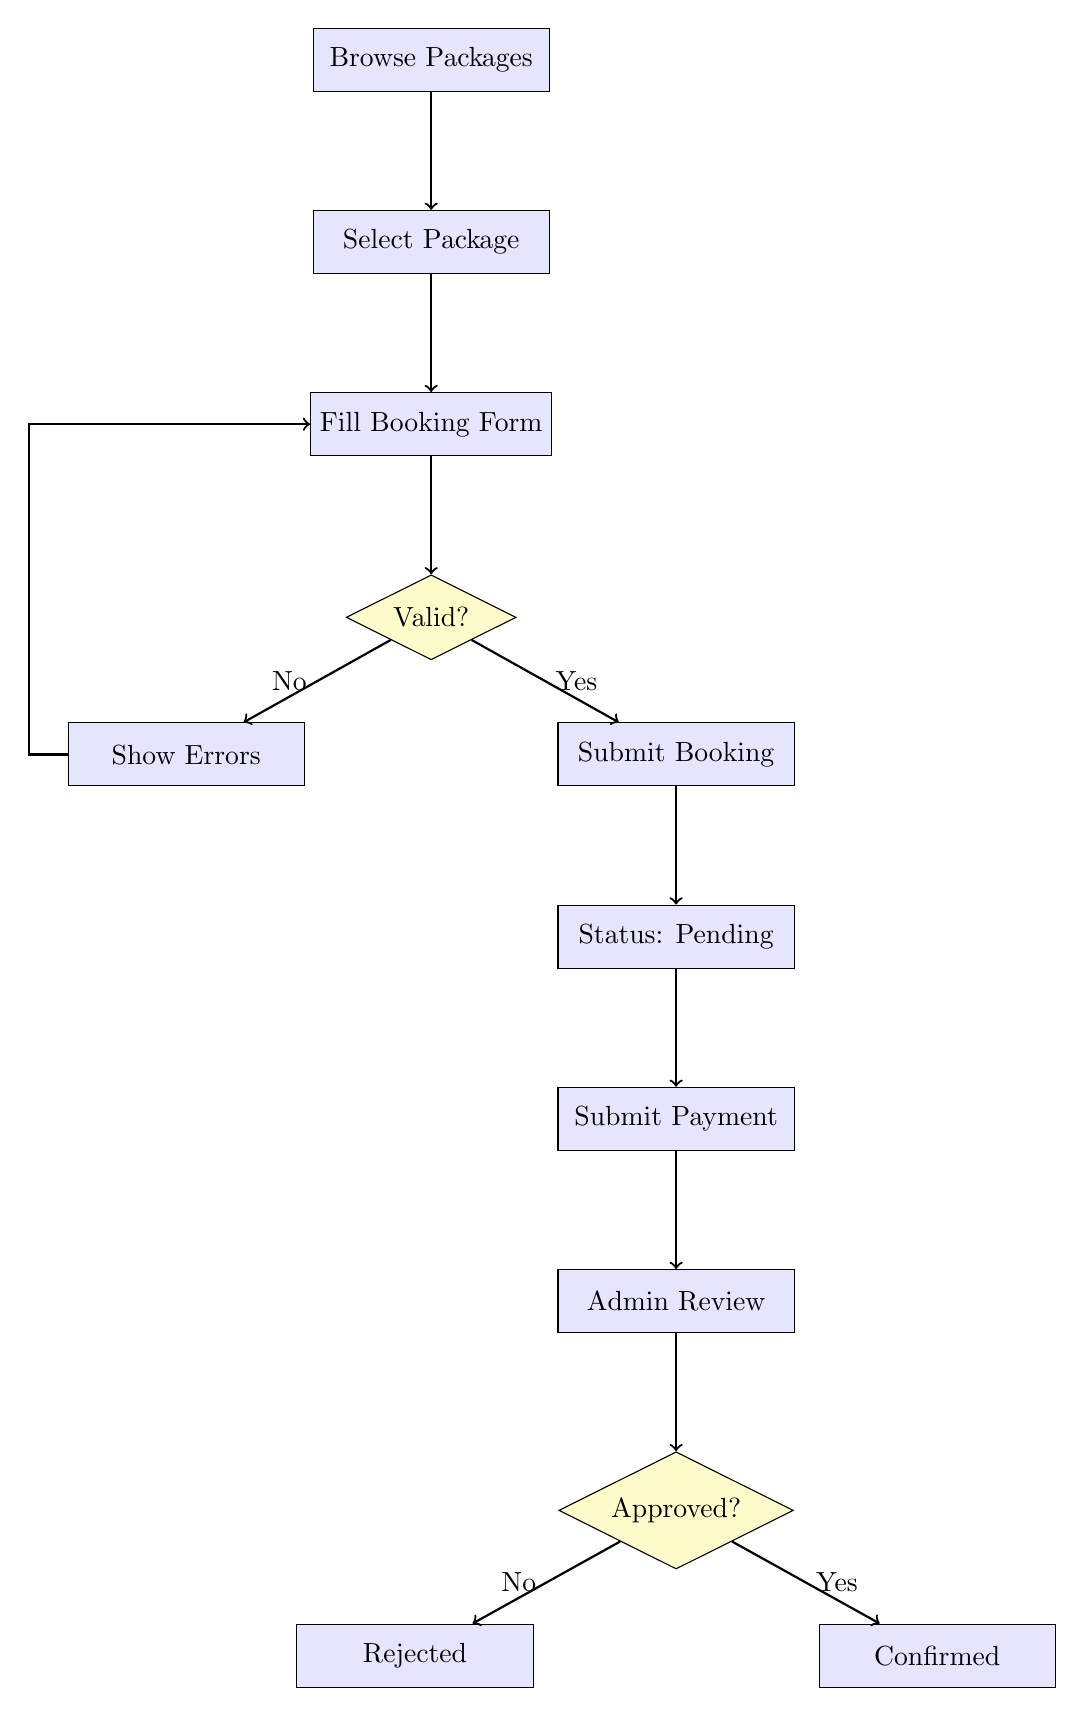
\begin{tikzpicture}[
    node distance=1.5cm,
    box/.style={rectangle, draw, minimum width=3cm, minimum height=0.8cm, align=center, fill=blue!10},
    decision/.style={diamond, draw, aspect=2, fill=yellow!20},
    arrow/.style={->, thick}
]
    \node[box] (browse) {Browse Packages};
    \node[box, below=of browse] (select) {Select Package};
    \node[box, below=of select] (fill) {Fill Booking Form};
    \node[decision, below=of fill] (validate) {Valid?};
    \node[box, below left=of validate] (error) {Show Errors};
    \node[box, below right=of validate] (submit) {Submit Booking};
    \node[box, below=of submit] (pending) {Status: Pending};
    \node[box, below=of pending] (payment) {Submit Payment};
    \node[box, below=of payment] (admin) {Admin Review};
    \node[decision, below=of admin] (approve) {Approved?};
    \node[box, below right=of approve] (confirmed) {Confirmed};
    \node[box, below left=of approve] (rejected) {Rejected};
    
    \draw[arrow] (browse) -- (select);
    \draw[arrow] (select) -- (fill);
    \draw[arrow] (fill) -- (validate);
    \draw[arrow] (validate) -- node[left] {No} (error);
    \draw[arrow] (validate) -- node[right] {Yes} (submit);
    \draw[arrow] (error) -- ++(-2,0) |- (fill);
    \draw[arrow] (submit) -- (pending);
    \draw[arrow] (pending) -- (payment);
    \draw[arrow] (payment) -- (admin);
    \draw[arrow] (admin) -- (approve);
    \draw[arrow] (approve) -- node[right] {Yes} (confirmed);
    \draw[arrow] (approve) -- node[left] {No} (rejected);
\end{tikzpicture}
\caption{Package Booking Workflow}
\label{fig:booking-flow}
\end{figure}

\subsection{Booking Status Management}
\begin{lstlisting}[language=Python, caption=Booking Status Choices]
STATUS_CHOICES = [
    ('pending', 'Pending'),
    ('approved', 'Approved'),
    ('rejected', 'Rejected'),
    ('cancelled', 'Cancelled'),
]

PAYMENT_STATUS_CHOICES = [
    ('pending', 'Pending Verification'),
    ('verified', 'Verified'),
    ('rejected', 'Rejected'),
]
\end{lstlisting}

\section{Admin Functions}

\subsection{Admin Dashboard Features}
\begin{itemize}[noitemsep]
    \item View all pending bookings
    \item Approve or reject booking requests
    \item Verify payment submissions
    \item Manage tour packages (CRUD operations)
    \item Handle travel requests from students
    \item View and respond to contact messages
\end{itemize}

\subsection{Admin Views}
\begin{lstlisting}[language=Python, caption=Admin Booking Management]
@staff_member_required
def admin_package_bookings(request):
    """Admin view for managing all package bookings"""
    bookings = PackageBooking.objects.all().order_by('-created_at')
    
    # Filter by status if provided
    status_filter = request.GET.get('status', '')
    if status_filter:
        bookings = bookings.filter(status=status_filter)
    
    return render(request, 'admin_package_bookings.html', {
        'bookings': bookings,
        'status_filter': status_filter
    })
\end{lstlisting}

\section{URL Routing}
The system uses Django's URL dispatcher to route requests to appropriate views.

\begin{lstlisting}[language=Python, caption=Main URL Configuration]
urlpatterns = [
    # Basic pages
    path('', home, name='home'),
    path('about/', about, name='about'),
    path('contact/', contact, name='contact'),
    
    # Authentication URLs
    path('register/', register, name='register'),
    path('login/', CustomLoginView.as_view(), name='login'),
    path('logout/', custom_logout, name='custom_logout'),
    
    # Booking URLs
    path('packages/', study_tour_detail, name='packages'),
    path('book-study-tour/', book_study_tour, name='book_study_tour'),
    path('my-bookings/', my_bookings, name='my_bookings'),
    
    # Admin URLs
    path('admin/bookings/', admin_booking_management, 
         name='admin_booking_management'),
    path('admin/', admin.site.urls),
]
\end{lstlisting}

%============================================
% CHAPTER 5: FRONTEND TEMPLATES
%============================================
\chapter{Frontend Templates}

\section{Template Inheritance}
Django templates use inheritance to maintain consistency across pages.

\subsection{Base Template Structure}
The \texttt{base.html} template provides the common structure for all pages:
\begin{itemize}[noitemsep]
    \item Navigation bar with role-based links
    \item Content block for page-specific content
    \item Footer section
    \item JavaScript and CSS includes
\end{itemize}

\section{Key Templates}

\begin{table}[H]
\centering
\caption{Template Files Description}
\label{tab:templates}
\begin{tabular}{|l|p{8cm}|}
\hline
\textbf{Template} & \textbf{Description} \\
\hline
base.html & Base template with common layout \\
home.html & Landing page with featured tours \\
login.html & User login page \\
register.html & User registration page \\
packages.html & Tour packages listing \\
book\_package.html & Package booking form \\
my\_bookings.html & User's booking history \\
my\_package\_bookings.html & Package booking details \\
admin\_bookings.html & Admin booking management \\
admin\_package\_bookings.html & Admin package booking view \\
travel\_request\_form.html & Travel request submission \\
my\_travel\_requests.html & User's travel requests \\
admin\_travel\_requests.html & Admin travel request management \\
contact.html & Contact form/message inbox \\
about.html & About page \\
spot\_detail.html & Tourist spot details \\
\hline
\end{tabular}
\end{table}

%============================================
% CHAPTER 6: API ENDPOINTS
%============================================
\chapter{API Endpoints}

\section{Available Endpoints}

\begin{longtable}{|l|l|p{5cm}|l|}
\caption{API Endpoints Reference} \label{tab:api-endpoints} \\
\hline
\textbf{Endpoint} & \textbf{Method} & \textbf{Description} & \textbf{Auth} \\
\hline
\endfirsthead
\hline
\textbf{Endpoint} & \textbf{Method} & \textbf{Description} & \textbf{Auth} \\
\hline
\endhead
\hline
\endfoot
\hline
\endlastfoot

\texttt{/} & GET & Home page & No \\
\texttt{/register/} & GET, POST & User registration & No \\
\texttt{/login/} & GET, POST & User login & No \\
\texttt{/logout/} & GET & User logout & Yes \\
\texttt{/packages/} & GET & List packages & No \\
\texttt{/packages/book/<id>/} & GET, POST & Book package & Yes \\
\texttt{/my-bookings/} & GET & User bookings & Yes \\
\texttt{/admin/bookings/} & GET & Admin bookings & Admin \\
\texttt{/admin/bookings/approve/<id>/} & POST & Approve booking & Admin \\
\texttt{/admin/bookings/reject/<id>/} & POST & Reject booking & Admin \\
\texttt{/payment/submit/<id>/} & POST & Submit payment & Yes \\
\texttt{/payment/verify/<id>/} & POST & Verify payment & Admin \\
\texttt{/travel-request/submit/} & POST & Submit request & Yes \\
\texttt{/travel-request/admin/} & GET & Admin requests & Admin \\
\texttt{/contact/} & GET, POST & Contact page & No \\
\texttt{/api/available-slots/<id>/} & GET & Get slots & Yes \\
\end{longtable}

%============================================
% CHAPTER 7: DEPLOYMENT GUIDE
%============================================
\chapter{Deployment Guide}

\section{Local Development Setup}

\subsection{Step 1: Clone the Repository}
\begin{lstlisting}[language=bash]
git clone <repository-url>
cd os_djangopro
\end{lstlisting}

\subsection{Step 2: Create Virtual Environment}
\begin{lstlisting}[language=bash]
# Windows
python -m venv venv
venv\Scripts\activate

# Linux/Mac
python3 -m venv venv
source venv/bin/activate
\end{lstlisting}

\subsection{Step 3: Install Dependencies}
\begin{lstlisting}[language=bash]
pip install -r requirements.txt
\end{lstlisting}

\subsection{Step 4: Database Setup}
\begin{lstlisting}[language=bash]
python manage.py makemigrations
python manage.py migrate
python manage.py createsuperuser
\end{lstlisting}

\subsection{Step 5: Run Development Server}
\begin{lstlisting}[language=bash]
python manage.py runserver
\end{lstlisting}

Access the application at \texttt{http://127.0.0.1:8000/}

\section{Production Deployment}

\subsection{PythonAnywhere Deployment}
PythonAnywhere is recommended for Django hosting due to its simplicity.

\subsubsection{Step 1: Create Account}
\begin{enumerate}
    \item Sign up at \url{https://www.pythonanywhere.com}
    \item Choose a free or paid plan
\end{enumerate}

\subsubsection{Step 2: Upload Code}
\begin{lstlisting}[language=bash]
# In PythonAnywhere bash console
git clone <your-repo-url>
cd os_djangopro
\end{lstlisting}

\subsubsection{Step 3: Create Virtual Environment}
\begin{lstlisting}[language=bash]
mkvirtualenv --python=/usr/bin/python3.10 myenv
pip install -r requirements.txt
\end{lstlisting}

\subsubsection{Step 4: Configure Web App}
\begin{enumerate}
    \item Go to Web tab
    \item Create new web app
    \item Choose Manual Configuration
    \item Set Python version to 3.10
\end{enumerate}

\subsubsection{Step 5: WSGI Configuration}
Edit the WSGI file:
\begin{lstlisting}[language=Python]
import os
import sys

path = '/home/yourusername/os_djangopro'
if path not in sys.path:
    sys.path.append(path)

os.environ['DJANGO_SETTINGS_MODULE'] = 'os_djangopro.settings'

from django.core.wsgi import get_wsgi_application
application = get_wsgi_application()
\end{lstlisting}

\subsubsection{Step 6: Static Files}
Configure static files in Web tab:
\begin{itemize}
    \item URL: \texttt{/static/}
    \item Directory: \texttt{/home/yourusername/os\_djangopro/staticfiles/}
    \item URL: \texttt{/media/}
    \item Directory: \texttt{/home/yourusername/os\_djangopro/media/}
\end{itemize}

\subsubsection{Step 7: Collect Static Files}
\begin{lstlisting}[language=bash]
python manage.py collectstatic
\end{lstlisting}

\subsection{Heroku Deployment}
\subsubsection{Prerequisites}
\begin{itemize}
    \item Heroku CLI installed
    \item Git repository initialized
\end{itemize}

\subsubsection{Required Files}
\textbf{Procfile:}
\begin{lstlisting}
web: gunicorn os_djangopro.wsgi
\end{lstlisting}

\textbf{runtime.txt:}
\begin{lstlisting}
python-3.10.12
\end{lstlisting}

\subsubsection{Deployment Commands}
\begin{lstlisting}[language=bash]
heroku login
heroku create your-app-name
git push heroku main
heroku run python manage.py migrate
heroku run python manage.py createsuperuser
\end{lstlisting}

\section{Avoiding Common Conflicts}

\subsection{Database Conflicts}
\begin{itemize}
    \item Always run \texttt{makemigrations} before \texttt{migrate}
    \item Never delete migration files manually in production
    \item Use \texttt{python manage.py showmigrations} to check status
\end{itemize}

\subsection{Static Files Conflicts}
\begin{lstlisting}[language=Python]
# settings.py - Production settings
DEBUG = False
STATIC_ROOT = BASE_DIR / 'staticfiles'
STATICFILES_STORAGE = 'whitenoise.storage.CompressedManifestStaticFilesStorage'
\end{lstlisting}

\subsection{URL Conflicts}
Ensure unique URL patterns:
\begin{lstlisting}[language=Python]
# Avoid conflicts by using prefixes
path('admin/', admin.site.urls),  # Django admin
path('admin-bookings/', admin_package_bookings, 
     name='admin_package_bookings'),  # App admin
\end{lstlisting}

\subsection{Environment Variables}
\begin{lstlisting}[language=Python]
# settings.py
import os

SECRET_KEY = os.getenv('SECRET_KEY', 'fallback-secret-key')
DEBUG = os.getenv('DEBUG', 'True') == 'True'
ALLOWED_HOSTS = ['yourdomain.com', 'localhost', '127.0.0.1']
\end{lstlisting}

\section{Security Checklist for Production}
\begin{enumerate}
    \item Set \texttt{DEBUG = False}
    \item Generate a strong \texttt{SECRET\_KEY}
    \item Configure \texttt{ALLOWED\_HOSTS}
    \item Enable HTTPS
    \item Set secure cookie settings
    \item Configure CSRF protection
    \item Use environment variables for sensitive data
\end{enumerate}

\begin{lstlisting}[language=Python]
# Production security settings
SECURE_BROWSER_XSS_FILTER = True
SECURE_CONTENT_TYPE_NOSNIFF = True
SESSION_COOKIE_SECURE = True
CSRF_COOKIE_SECURE = True
X_FRAME_OPTIONS = 'DENY'
\end{lstlisting}

%============================================
% CHAPTER 8: USER GUIDE
%============================================
\chapter{User Guide}

\section{Student Features}

\subsection{Registration}
\begin{enumerate}
    \item Navigate to the registration page
    \item Select "Student" as role
    \item Fill in required fields:
    \begin{itemize}
        \item Username
        \item Full Name
        \item Email
        \item Student ID
        \item Department
        \item Session
        \item Password
    \end{itemize}
    \item Click "Register"
\end{enumerate}

\subsection{Booking a Package}
\begin{enumerate}
    \item Login to your account
    \item Browse available packages
    \item Select desired package
    \item Fill in booking details
    \item Submit booking request
    \item Wait for admin approval
    \item Submit payment via bKash
    \item Check booking status in "My Bookings"
\end{enumerate}

\subsection{Submitting Travel Request}
\begin{enumerate}
    \item Navigate to "Travel Request"
    \item Fill in place details
    \item Specify preferred date and budget
    \item Submit request
    \item Track status in "My Travel Requests"
\end{enumerate}

\section{Admin Features}

\subsection{Managing Packages}
\begin{enumerate}
    \item Login as admin
    \item Navigate to package management
    \item Add/Edit/Delete packages
    \item Set categories and pricing
\end{enumerate}

\subsection{Booking Approval Process}
\begin{enumerate}
    \item View pending bookings
    \item Review student details
    \item Verify payment information
    \item Approve or reject booking
    \item Add admin notes if needed
\end{enumerate}

\subsection{Travel Request Management}
\begin{enumerate}
    \item View all pending requests
    \item Review request details
    \item Approve/Reject with response
    \item Convert to package if approved
\end{enumerate}

%============================================
% CHAPTER 9: TROUBLESHOOTING
%============================================
\chapter{Troubleshooting}

\section{Common Issues and Solutions}

\subsection{Migration Errors}
\textbf{Problem:} Migration conflicts or errors

\textbf{Solution:}
\begin{lstlisting}[language=bash]
# Reset migrations (development only)
python manage.py migrate --fake-initial

# Or recreate database
rm db.sqlite3
python manage.py makemigrations
python manage.py migrate
\end{lstlisting}

\subsection{Static Files Not Loading}
\textbf{Problem:} CSS/JS not loading in production

\textbf{Solution:}
\begin{lstlisting}[language=bash]
python manage.py collectstatic --noinput
\end{lstlisting}

Ensure WhiteNoise is configured properly in \texttt{settings.py}.

\subsection{Permission Denied Errors}
\textbf{Problem:} User cannot access certain pages

\textbf{Solution:}
\begin{itemize}
    \item Verify user is authenticated
    \item Check if user has correct role (staff/superuser)
    \item Review decorator requirements on views
\end{itemize}

\subsection{Image Upload Issues}
\textbf{Problem:} Images not uploading or displaying

\textbf{Solution:}
\begin{lstlisting}[language=Python]
# settings.py
MEDIA_URL = '/media/'
MEDIA_ROOT = BASE_DIR / 'media'

# urls.py (development)
from django.conf import settings
from django.conf.urls.static import static

urlpatterns += static(settings.MEDIA_URL, 
                      document_root=settings.MEDIA_ROOT)
\end{lstlisting}

%============================================
% APPENDIX
%============================================
\appendix
\chapter{Requirements File}
\begin{lstlisting}
Django==5.2.9
pillow==12.0.0
gunicorn==23.0.0
whitenoise==6.11.0
sqlparse==0.5.5
asgiref==3.11.0
\end{lstlisting}

\chapter{Environment Variables}
\begin{table}[H]
\centering
\caption{Required Environment Variables}
\begin{tabular}{|l|l|p{5cm}|}
\hline
\textbf{Variable} & \textbf{Example} & \textbf{Description} \\
\hline
SECRET\_KEY & random-string-here & Django secret key \\
DEBUG & False & Debug mode (True/False) \\
ALLOWED\_HOSTS & yourdomain.com & Allowed host names \\
\hline
\end{tabular}
\end{table}

\chapter{Database Schema SQL}
\begin{lstlisting}[language=SQL]
-- Generated from Django ORM
-- View with: python manage.py sqlmigrate app_name migration_name

CREATE TABLE "tourist_spots_tourpackage" (
    "id" integer NOT NULL PRIMARY KEY AUTOINCREMENT,
    "name" varchar(200) NOT NULL,
    "description" text NOT NULL,
    "image" varchar(100) NOT NULL,
    "price" decimal NOT NULL,
    "duration" varchar(100) NOT NULL,
    "destination" varchar(200) NOT NULL,
    "highlights" text NULL,
    "category" varchar(50) NOT NULL,
    "is_active" bool NOT NULL,
    "created_at" datetime NOT NULL,
    "updated_at" datetime NOT NULL,
    "created_by_id" integer NOT NULL REFERENCES "auth_user" ("id")
);
\end{lstlisting}

%============================================
% GLOSSARY
%============================================
\chapter*{Glossary}
\addcontentsline{toc}{chapter}{Glossary}

\begin{description}
    \item[Django] A high-level Python web framework
    \item[MVT] Model-View-Template architectural pattern
    \item[ORM] Object-Relational Mapping
    \item[CRUD] Create, Read, Update, Delete operations
    \item[WSGI] Web Server Gateway Interface
    \item[SQLite] Lightweight file-based database
    \item[bKash] Mobile payment service in Bangladesh
    \item[PK] Primary Key
    \item[FK] Foreign Key
    \item[ERD] Entity Relationship Diagram
    \item[EER] Enhanced Entity Relationship Diagram
\end{description}

%============================================
% REFERENCES
%============================================
\begin{thebibliography}{9}
\bibitem{django}
Django Software Foundation.
\textit{Django Documentation}.
\url{https://docs.djangoproject.com/}

\bibitem{python}
Python Software Foundation.
\textit{Python Documentation}.
\url{https://docs.python.org/3/}

\bibitem{pythonanywhere}
PythonAnywhere.
\textit{Deployment Documentation}.
\url{https://help.pythonanywhere.com/}

\bibitem{heroku}
Salesforce.
\textit{Heroku Django Deployment}.
\url{https://devcenter.heroku.com/articles/django-app-configuration}
\end{thebibliography}

\end{document}
